\chapter{Ejemplos Sencillos}
\label{cap.sencillos}

En este capítulo se aplicarán las ideas del capítulo anterior a ejemplos sencillos. Estudiaremos el operador $A = - \partial ^2 _x$ en el intervalo $[0,L]$ sometido a distintas condiciones de contorno. Calcularemos la {\it función-$\zeta$} para luego obtener la energía de vacío. 

En los tres primeros casos se considerará condiciones de contorno Dirichlet, Neumann y periódicas en ambos extremos. Luego conociendo sus autovalores  se calculara la {\it función-$\zeta$} exactamente. 

En el último ejemplo de este capítulo, se tomará una condición de contorno Dirichlet en un borde y Robin en el otro, de modo de introducir un parámetro externo con dimensiones. Se utilizarán tres técnicas distintas para estudiar la {\it función-$\zeta$}: el desarrollo asintótico de los autavalores, una representacion en el plano complejo  y el heat-kernel.

\section{Condiciones de contorno Dirichlet,Neumann y periódicas}
\label{sec.Dirichlet}

En esta sección se estudiarán el espectro y las energía de vacío del operador $A = - \partial ^2 _x$ en el intervalo $[0,L]$ bajo condiciones de contorno Dirichlet,Neumann y periódicas:\\

\textbf{Condiciones de contorno Dirichlet}


Consideremos primeramente el operador $A$ dado por
\begin{equation}
\begin{aligned}
	A \phi (x) &= - \partial _x ^2 \phi (x) \\[10pt]
    \phi (0) &= \phi(L) = 0 
    \, .
\end{aligned}
\end{equation}

Sus autovalores y autofunciones normalizadas son

\begin{equation}
\begin{aligned}
	\phi _n (x) &= \sqrt{\frac{2}{L}} \sin( \frac{n \pi x}{L} ) \\[10pt]
	\lambda ^2 _n  &= \left( \frac{n \pi }{L} \right) ^2 \, \, \, \, \, n = 1,2,3, \, ...
\end{aligned}
\end{equation}

la {\it función-$\zeta$} queda determinada por

\begin{equation}
\begin{aligned}
\zeta  (s) &= 
\sum _{n=1} ^{\infty} \left( \frac{\lambda _n }{\mu }  \right) ^{-2s}  \\[10pt]
&= \left(  \frac{\pi}{L \mu} \right) ^{-2s}   \sum _{n=1} ^{\infty} n ^{-2s} = 
\left( \frac{\pi}{L \mu} \right) ^{-2s}  \zeta _R (2s) \, . \\[10pt]
\end{aligned}
\end{equation}

Donde $\zeta _R$ es la función zeta de Riemann definida en \ref{rieman-zeta-def}, en el apendice [CITAR] se demuestra  que $\zeta _R (-1) = -1/12$. 

Por lo tanto resulta que $\zeta$ es regular en $s=-\frac{1}{2}$, siendo la energía de vacío

\begin{equation}\label{eq.energia.dirichlet}
\begin{array}{c}
E _0 = - \frac{\pi}{24 L} \, ,
\end{array}
\end{equation}


Como la energía de vacío crece con $L$, el efecto Casimir implica una fuerza
atractiva entre los extremos del intervalo en el cual está confinado el campo
escalar. Notar que, como la {\it función-$\zeta$} es regular en $s=-\frac{1}{2}$, el resultado no depende del parámetro de escala $\mu$.\\

\subsection*{Condiciones de contorno Neumann}


Consideremos ahora el operador $A$ dado por.

\begin{equation}
\begin{aligned}
	A \phi (x) &= - \partial _x ^2 \phi (x) \\[10pt]
    \phi ' (0) &= \phi ' (L) = 0 \, ,
\end{aligned}
\end{equation}
cuyos autovalores y autofunciones están dados por
\begin{equation}
\begin{aligned}
	\phi _0 (x) &= \sqrt{ \frac{1}{L} } \\[5pt]
	\phi _n (x)  &= \sqrt{\frac{2}{L}} \cos \left( \frac{n \pi x}{L} \right) 
	\, \, \, \, \, \, n \neq 0\\[5pt]
	\lambda ^2 _n  &= \left( \frac{n \pi }{L} \right) ^2 
	\, \, \, \, \, \,
	n = 0,1,2,3, \dots
	\\[5pt]
\end{aligned}
\end{equation}


Como el cálculo de la {\it función-$\zeta$} se realiza excluyendo los modos cero, la
energía de vacıío coincide con la calculada anteriormente para condiciones
de contorno Dirichlet.\\



\textbf{Condiciones de contorno periódicas}\\

Estudiemos ahora el mismo operador bajo condiciones de contorno periódicas
\begin{equation}
\begin{array}{c}
	A \phi (x) = - \partial _x ^2 \phi (x) \\[5pt]
    \phi (0) = \phi (L)  \\[5pt]
    \phi ' (0) = \phi ' (L) \, ,
\end{array}
\end{equation}
Este problema representa una partícula escalar confinada en un anillo $S ^1$ .
Los autovalores y autofunciones están dados por


\begin{align}
	\phi _{0} &= \sqrt{\frac{1}{L}} \\[5pt]
	\phi _{n} (x) &= \sqrt{\frac{2}{L}} \cos \left( \frac{2 n \pi x}{L} \right),
	\, \, \,  \psi _n (x) =\sqrt{\frac{2}{L}} \sin \left( \frac{n \pi x}{L} \right) 
	\, \, \, \, \, \, \, \, \, n \neq 0
	\\[5pt]
	\lambda ^2 _n  &= \left( \frac{2 n \pi }{L} \right) ^2 
	\, \, \, \, \, \, \, \, \,
	 n = 0,1,2,3, \dots
\end{align}

La {\it función-$\zeta$} resulta

\begin{equation}
\begin{aligned}
\zeta  (s) &= 
2 \sum _{n=1} ^{\infty} \left( \frac{\lambda _n}{\mu ^2} \right)^{-s} \\[5pt]
&=  2 \left( \frac{2 \pi}{L} \right) ^{-2s} \mu ^{2s} \sum _{n=1} ^{\infty} n ^{-2s} =  
2 \mu ^{2s} \left( \frac{2 \pi}{L} \right) ^{-2s} \zeta _R (2s)
\end{aligned}
\end{equation}
que al igual que en los casos anteriores es regular en $s=-1/2$. Obtenemos
entonces la energía de vacío
\begin{equation}
E _0 = - \frac{\pi}{6 L}
\end{equation}
Nuevamente, la energía crece con L, lo que señala una fuerza que tiende a
reducir el tamaño del anillo.

\section{Condiciones de Contorno Mixtas}


Introducimos ahora un parámetro $S$ con dimensiones, a partir de condiciones de contorno Robin en uno de los extremos del intervalo,

\begin{equation}
\begin{aligned}
    A \phi (x) &= - \partial ^2 _x \ \phi (x)  \\[5pt]
    \phi (0) &= 0 \\[5pt]
    \phi ' (L) + S \phi (L) &= 0 \, .
\end{aligned}
\end{equation}
Las autofunciones con autovalor no nulo son

\begin{equation}
\phi _n (x) = 
B _n \sin ( \lambda _n x ) \, .
\end{equation}
Donde $B_n$ es una constante de normalización. El espectro de autovalores no nulos $\lambda _n \neq 0 $ está dado por
\begin{align}
    \lambda _n   \cos( \lambda _n L) +  S \sin( \lambda _n L) &= 0
    \, . \label{autovalores2} 
\end{align}

Una vez obtenidos los autovalores, calcularemos la {\it función-$\zeta$}

\begin{equation}
    \zeta (s) =  \sum_{n = 1} ^{ \infty } \left( \frac{\lambda _n}{\mu } \right) ^ {-2 s} \, ,
    \tag{\ref{eq.casimir.mu}}
\end{equation}

la dificultad está en que las ecuación (\ref{autovalores2}) no provee una solución explícita para $\lambda _n$. Para estudiar la  {\it función-$\zeta$} utilizaremos tres técnicas: la primera de ellas consiste en obtener un desarrollo asintótico de los autovalores, la segunda utiliza una representación integral en el plano complejo de la {\it función-$\zeta$}, la tercera se basa en la relación con el {\it heat-kernel}. 

\subsection{Desarrollo Asintótico de los autovalores}{\label{seq.asin}}

Primeramente, definimos variables adimensionales $\tau _n = \lambda _n L $ y $\theta = S L $, de modo que la ecuación (\ref{autovalores2}) se puede expresar de la forma

\begin{equation}
    \tan (\tau _n) + \frac{\tau _n}{\theta} = 0
    \label{eq.asintota}
\end{equation}
En la figura \ref{fig:Dibujo1} están graficados los dos terminos de \ref{eq.asintota}. Puede verse que los autovalores $\tau _n$ tienden a las asíntotas verticales de $ \tan ( \tau ) $ a medida que $\tau _n$ crece. Por consiguiente, escribimos para los autovalores $\tau _n$ 
\begin{equation}
\begin{aligned}
    & \tau _n = n \pi + \frac{\pi}{2} + \epsilon _n \\[5pt]
    & \lim \limits_{ n \rightarrow \infty} \epsilon _n = 0 \\
\end{aligned}
\label{eq.mu}
\end{equation}
\begin{figure}
    \centering
    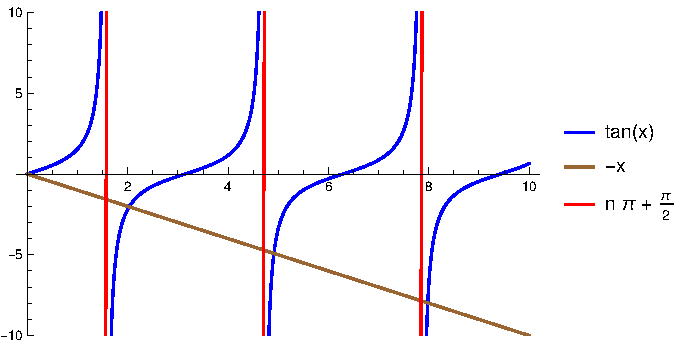
\includegraphics[scale=0.6]{Dibujo.pdf}
    \caption{En este ejemplo, se puede ver que la intersección entre $ \tan(x)$ y $-x$ tiende a las asíntotas verticales de $\tan (x) $, el mismo comportamiento se aprecia para cualquier recta de la forma $- a x$.}
    \label{fig:Dibujo1}
\end{figure}
Remplazando esta expresión en (\ref{autovalores2}),

\begin{equation}
\begin{aligned}
    \sin \left( n \pi + \frac{\pi}{2} + \epsilon _n \right) = -
    \frac{n \pi + \frac{\pi}{2} + \epsilon _n}{\theta} \cos \left( n \pi + \frac{\pi}{2} + \epsilon _n\right)
    \, ,
\end{aligned}
\end{equation}
podemos obtener un desarrollo de $\epsilon _n$ en potencias negativas del indice $n$. Para ello, desarrollamos esta ecuación para valores pequeños de $\epsilon _n$,   
\begin{equation}
    1 = 
    \sum _{p=0} ^{\infty} (-1) ^p     \left[
   	\left( \frac{1}{\theta (2p+1)!  } + \frac{1}{(2p+2)!} \right) \epsilon _n ^{2p+2 } +
  	\frac{n \pi + \frac{\pi}{2}}{\theta (2p+1)! }   \epsilon _n ^{2p+1} 			\right]
  	\, .
\label{igualdad epsilon}
\end{equation}
Esta expresión muestra que $\epsilon _n$ admite un desarrollo de la forma

\begin{equation}
    \epsilon _n = 
    \frac{\epsilon ^{(1)}}{n}  + 
    \frac{\epsilon ^{(2)}}{n ^2}  + 
    \frac{\epsilon ^{(3)}}{n ^3}  + ...
\label{eq.epsilon}
\end{equation}
Reemplazando este desarrollo en (\ref{igualdad epsilon}), e igualando orden a orden, obtenemos para los primeros términos
\begin{equation}
    \epsilon _n = \frac{\theta}{n \pi} 
     - \frac{ \theta}{2 \pi n ^2 } + O \left( n ^{-3}\right) 
     \, .
\label{epsilons}
\end{equation}
La  {\it función-$\zeta$} puede entonces escribirse
\begin{equation}
\begin{aligned}
    \zeta  (s) &=  
    \sum _{n=1} ^{\infty} 
    \left( \frac{\lambda _n }{\mu } 
    	\right) ^ {- 2s}  \\
    &=
    \mu ^{2s} \sum _{n=1} ^{\infty} 
    \left(
	\frac{n \pi}{L } + 
    \frac{\pi}{2 L } +
    \frac{\gamma}{n \pi } -
    \frac{\gamma}{2 \pi n ^2   } +
    O \left(  n^{-3} \right) 
    \right) ^{-2 s}  \\[5pt]
    &= \left( \frac{L \mu }{\pi} \right) ^{2s}    
    \sum _{n=1} ^{\infty} 
    n ^{- 2 s} 
    \left(
    1 +     
    \underbrace{
        \frac{1}{2 n} + 
        \frac{L \gamma}{n^2 \pi ^2} -
        \frac{L \gamma}{2 n ^3 \pi ^2} } 
        _{ \chi _n} +
        O \left(n ^{-4} \right)  
    \right ) ^{-2 s}
    \, .
\end{aligned}
\end{equation}

De manera consistente con los términos  $ O (n ^{-4})$ que no hemos calculado, desarrollamos el binomio para pequeños valores de $\chi _n$ hasta el orden cúbico,


\begin{align}
\zeta  (s) &= 
\left( \frac{L \mu }{\pi} \right) ^{2 s}
\sum _{n=1} ^{\infty}
  n  ^{-2 s} \times \\[5pt]
& \times   \ \Bigg(
	1 - 
	2 s \chi _n +  s(2s+1) \frac{\chi _n ^2}{2} - 
	\frac{2}{3} s(2s+1)(s+1) \chi _n ^3  + O \left( n ^{-4} \right) \Bigg)
	\, ,
	\nonumber
\end{align}

La {\it función-$\zeta$} puede entonces escribirse en términos de la función zeta de Riemann $\zeta _R (s)$


\begin{equation}
\begin{aligned}
    \zeta  (s) &= \left( \frac{L \mu }{\pi} \right) ^{2s} . \\[5pt]
	& \Bigg(
		\zeta _R ( 2 s ) -
		s \zeta _R ( 2s+1 ) +
		 s \left( \frac{1}{4} + \frac{s}{2} - \frac{2 L  \gamma}{\pi ^2} \right) \zeta _R (2s +2 ) - \\[5pt]
		 &  \left(  
					\frac{s(s+1) ( \pi ^2 + 2 \pi ^2 s - 24 L \gamma)}{12 \pi ^2 }
		 			\right) \zeta _R (2s+3)
		+ \sum _{n=1} ^{\infty} n ^{-2s} O ( n ^{-4})
		\Bigg)
		\, ,
\end{aligned}
\end{equation}
donde cada término $\sum _{n=1} ^{\infty} n ^{-2s} O ( n ^{-p})$ será proporcional a $\zeta _R (2s+p)$, que es una función meroforma con polo simple en $s = \frac{1}{2} - \frac{p}{2}$.
Por lo tanto los polos de $\zeta (s)$ están dados por el polo simple de $\zeta _R (s)$. De esta manera, se muestra que $\zeta (s)$ posee polos simples en semi-enteros negativos, de acuerdo con (\ref{eq.ceros.zeta}). El desarrollo hasta orden $O(n^{-3})$ que hemos calculado para los autovalores permite obtener los residuos correspondientes a los siguientes polos.


\begin{equation}
\begin{aligned}
\left(1- \frac{1}{2} \right) \zeta  (s)| _{s=\frac{1}{2}} &= 
\frac{L \mu }{2 \pi } \\[5pt]
s \zeta  (s) |_{s=0} &= \ 0 \\[5pt]
\left( s + \frac{1}{2} \right)\zeta  (s) | _{s=-\frac{1}{2}} &= \frac{\gamma}{2 \pi  } \\[5pt]
(s+1) \zeta (s) |_{s=-1} &=  0
\, ,
\\[5pt]
\end{aligned}
\label{eq.polos.asin}
\end{equation}



\subsection{Representación integral de la función $\zeta$}
{\label{sec.complejo}}

En la sección \ref{seq.asin} se calculó un desarrollo de los autovalores y luego se
los utilizó en la definición (\ref{def.adim}) para obtener
la estructura de polos de la función $\zeta$. En este capítulo estudiaremos la
estructura analítica de $\zeta (s)$ de una manera alternativa, que será de utilidad
más adelante.

Supongamos que los autovalores $\lambda ^2 _n$ están definidos por una expresión de
la forma $f ( \lambda ^2 _ n ) = 0$ y que $\lambda ^2 _n$  son ceros simples de la función analítica $f (z)$.
En ese caso, la función $( \log f (z))'$ tiene polos simples en $\lambda ^2 _n$ con residuo 1.
Utilizando el teorema de los residuos, la función $\zeta (s)$ se puede representar
como una integral en el plano complejo cuyo camino de integración $C$
encierra los ceros de $f (z)$ (véase la figura \ref{fig:contorno}),
\begin{equation}
\begin{aligned}
   \zeta  (s) &=  \sum _{n=1} ^{\infty} \left( \frac{\lambda _n}{\mu} \right) ^{-2s} 
   =  
   \frac{1}{2 \pi i} \int _{C} \frac{f'(z)}{f(z)} \left( \frac{z}{\mu} \right) ^{-2s} dz 
\end{aligned}
\label{asd}
\end{equation}
En el problema que estamos considerando $f(z) = z \cos Lz + \gamma \sin Lz$ (ver (\ref{autovalores2})). Reemplazando en la representación integral obtenemos


\begin{equation}
	\zeta  (s) = 
    \frac{\mu ^{2s}}{2 \pi i} \int _{C}
    \frac{ \cos (L z) \left(L + \frac{1}{\gamma} \right) - \sin(L z) \frac{z L}{\gamma}
    }
    { \cos(L z) \frac{z}{\gamma} + \sin(L z)
    }
     z  ^{-2 s} dz  \, .
\end{equation}

\begin{figure*}[t!]
    \centering
    \begin{subfigure}[t]{0.3\textwidth}
        \centering
        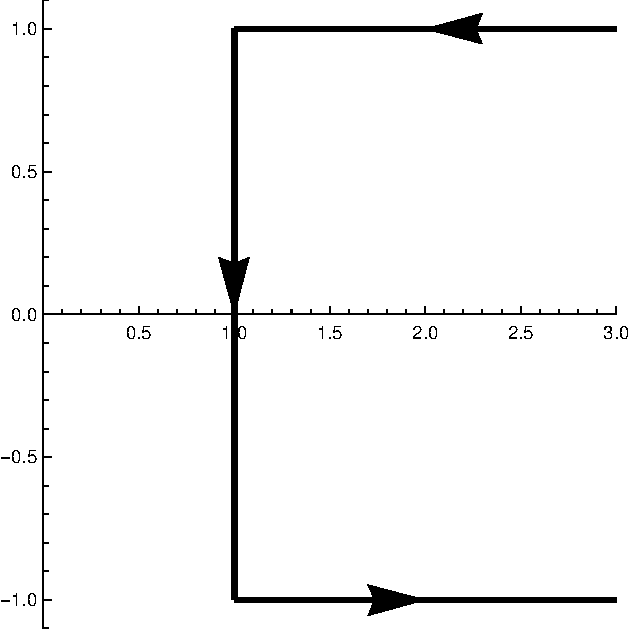
\includegraphics[height=1.2in]{Camino.pdf}
        \caption{}
        \label{fig.izquierda}
    \end{subfigure}%
    ~ 
    \begin{subfigure}[t]{0.3\textwidth}
        \centering
        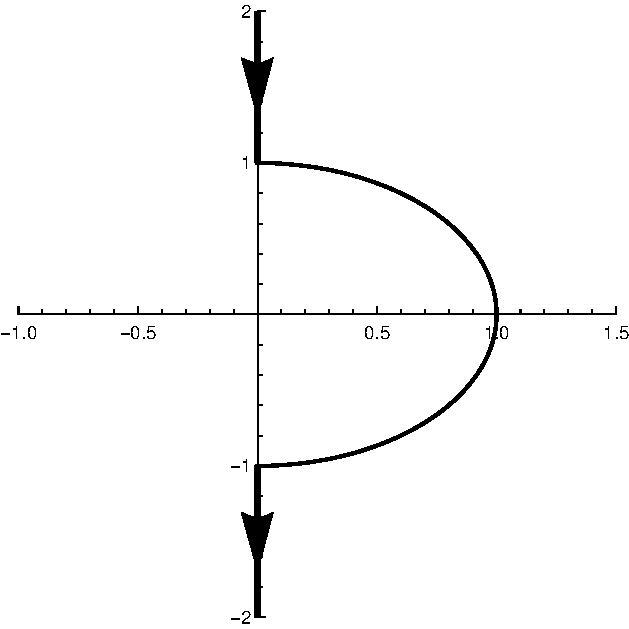
\includegraphics[height=1.2in]{Camino2.pdf}
        \caption{}
        \label{fig.derecha}
    \end{subfigure}
    ~
    \begin{subfigure}[t]{0.3\textwidth}
        \centering
        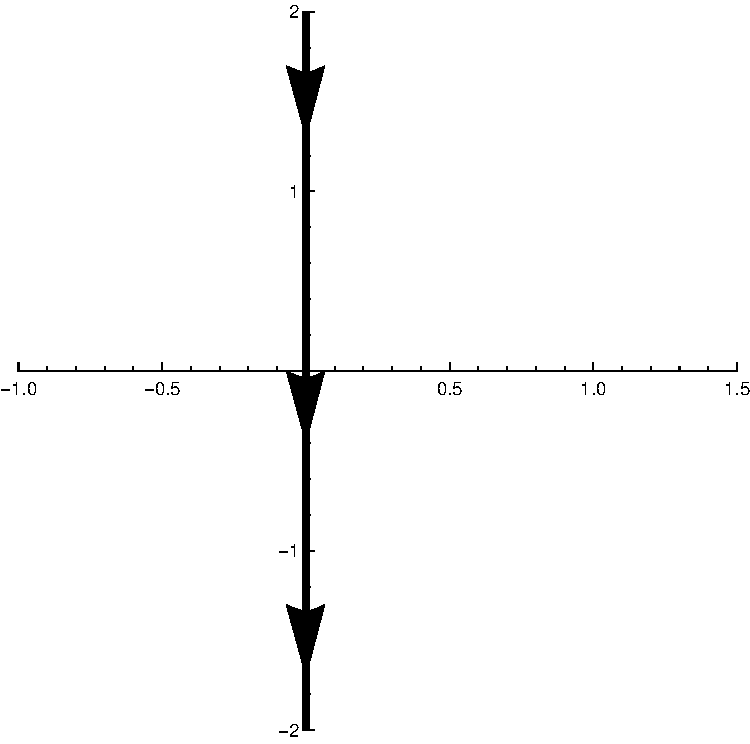
\includegraphics[height=1.2in]{Camino3.pdf}
        \caption{}
        \label{fig.derecha.derecha}
    \end{subfigure}
    \caption{Estos caminos son los tenidos en cuenta para representar a la {\it función-$\zeta$} como una integral en el plano complejo.}
\label{fig:contorno}
\end{figure*}


Se va a utilizar el camino de la figura \ref{fig.derecha}, el cual se puede descomponer en 3 integrales, una angular que es regular $ \forall s$ y por lo tanto no aporta a la estructura de polos, y dos rectas las cuales se van a parametrizar de la forma $z = \pm i  t$. 

Para las ramas de $z= i t$ y $z=- i t$ se obtienen respectivamente
\begin{equation}\label{eq.tirados}
\begin{aligned}
\frac{e ^{-i \pi s}}{2 \pi i} \int _{\infty} ^{1} 
	\frac{(1+L \gamma) \left( e^{L t} - e ^{- L t} \right) +
			(L t) \left( e ^{L t} - e^{- L t} \right)
			}
			{\gamma \left( e ^{L t} - e ^{- L t} \right) + 
			t \left( e ^{L t} - e ^{-L t} \right)}
			t ^{-2s} dt \\[7pt]
\frac{e ^{i \pi s}}{2 \pi i} \int _{1} ^{\infty} 
	\frac{(1+L \gamma) \left( e^{L t} - e ^{- L t} \right) +
			(L t) \left( e ^{L t} - e^{- L t} \right)
			}
			{\gamma \left( e ^{L t} - e ^{- L t} \right) + 
			t \left( e ^{L t} - e ^{-L t} \right)}
			t ^{-2s} dt
			\, .
\end{aligned}
\end{equation}
A partir de estas expresiones, teniendo en cuenta que los términos exponenciales decrecientes no contribuyen a la estructura de polos, la {\it función-$\zeta$} queda expresada como

\begin{equation}
	\zeta  (s) = 
    \frac{ \sin (\pi s) \mu ^{2s}}{ \pi } 
    \int _1 ^{\infty} 
    t^{-2s}
    \left(
    	L + 
	    \underbrace
    	{
		\frac{1}{\gamma + t}   
		} _{\chi} 
	\right)
    dt  \,  ,
\label{contorno}
\end{equation}
en $\chi$ se puede sacar factor común $t$ y utilizar la serie geométrica para obtener

\begin{equation}
    \chi =   \sum _{m=0} ^{\infty} \frac{(-1) ^{m} \gamma ^{m} }{t ^{m+1}}
    \, ,
\label{eq:chi}
\end{equation}
pudiendo entonces integrar termino a termino, el resultado final está dado por
\begin{equation}\label{eq.seta}
    \zeta  (s) = 
    \frac{ \sin(\pi s) \mu ^{2s }}{\pi } 
    \left(
    \frac{L}{2s-1} + 
    \sum _{m=0} ^{\infty}
    \frac{(-1) ^{m} \gamma ^{m} }{2s+m}
    \right) \, .
\end{equation}
Se puede ver que la {\it función-$\zeta$} tiene polos simples en $s=1/2$ y en los semienteros negativos, la estructura de polos queda determinada por
\begin{equation}
\begin{aligned}
\left(s-\frac{1}{2} \right) \zeta(s) |_{s=\frac{1}{2}} &= \frac{L \mu }{2 \pi}   \\
\left( s + n + \frac{1}{2} \right)
\zeta (s ) |_{s= -n - \frac{1}{2}}  &= \frac{ (-1) ^n \gamma ^{2n+1}  }{2 \pi \mu ^{2n + 1}} 
\, .
\end{aligned}
\label{eq.polos.complejo}
\end{equation}


Lo cual coincide a los primeros ordenes con (\ref{eq.polos.asin}) y está en concordancia  con (\ref{eq.ceros.zeta}).

Utilizando esta técnica se puede sacar la estructura entera de polos de la {\it función-$\zeta (s)$}, para calcular la parte finita hay que tener en cuenta la parte angular de (\ref{asd}), y los términos exponenciales tirados en (\ref{eq.tirados}) para llegar a (\ref{contorno}).


\subsection{Uso del Heat-Kernel}

En las secciones \ref{sec.complejo} y \ref{seq.asin} se utilizaron técnicas para aproximar la {\it función-$\zeta$}, obteniendo la estructura de polos. En esta sección se hará uso del resultado general (\ref{eq.heat.expansion}) para obtener los polos de la {\it función-$\zeta$}.

En la ecuación (\ref{coef}) están presentados los primeros términos de Seeley-DeWitt para un operador con borde, en estas condiciones: variedad unidimensional, sin curvatura, y condición de contorno Robin en un extremo y Dirichlet en el otro, los coeficientes de Seeley-DeWitt quedan expresados como {\red(¿es evidente el valor de C1? ¿por qué es negativo? ¿de dónde sale el signo de C2?)}:


\begin{equation}
\begin{aligned}
C _0 &=  \frac{L \mu}{\sqrt{4 \pi} }\\
C _1 &=  -2 \\
C _2 &= - \frac{\gamma}{\mu \sqrt{\pi} } \\
C _3 &= \frac{ \gamma ^2 }{2 \mu ^2 }
\end{aligned}
\end{equation}


Luego se utiliza la ecuación (\ref{losresi}) que relaciona los coeficientes de Seeley-DeWitt con los residuos de los polos de la función $\zeta$
\begin{equation}
\left. {\rm Res} \ \zeta  (s)  \right| _{s_n= \frac{m - n}{2}} =  
\frac{ C_n  (A) }{ {\Gamma ( \frac{m-n}{2}} ) }
\tag{\ref{losresi}}
\, ,
\end{equation}
teniendo en cuenta que $\Gamma (-1) = \Gamma (-2) = \infty$, los residuos de la función-$\zeta$ están dados por
\begin{equation}
\begin{aligned}
Res \  \zeta  (s)  | _{s=1/2} &= \frac{L \mu}{2 \pi} \\[5pt]
Res \  \zeta  (s)  | _{s=0} &= 0 \\[5pt]
Res \ \zeta (s) | _{s=-1/2} &= \frac{\gamma}{2 \pi \mu} \\[5pt]
Res \  \zeta  (s) | _{s=-1} &= 0 \, . \\[5pt]
\end{aligned}
\end{equation}


Lo cual coincide con (\ref{eq.polos.complejo}) y (\ref{eq.polos.asin}).

\subsection{Cálculo de la energía de vacío} 

La energía de vacío queda definida por la ecuación (\ref{eq.casimir.mu})

\begin{equation}
    E _0 = \frac{\mu }{2}  
    \zeta  \left( - 1/2 \right) 
    \tag{\ref{eq.casimir.mu}} \, ,
\end{equation}

Utilizando la expresión de $\zeta  (s )$ dada por (\ref{eq.seta}) en (\ref{eq.casimir.mu}) se obtiene para la energía de vacío

\begin{equation}
E _0 = \frac{1}{2} \left(
				\frac{\gamma}{2 \pi \left( s+\frac{1}{2} \right) }
				\right) + 
				\frac{\mu}{2} \ {\rm Regular}
\, .
\end{equation}
Donde la parte finita de la energía de vacío viene dada por la parte regular de la expresión anterior.
